\documentclass[border=2mm]{standalone}
\usepackage{tikz}
\usetikzlibrary{calc,patterns,angles,quotes}
\begin{document}
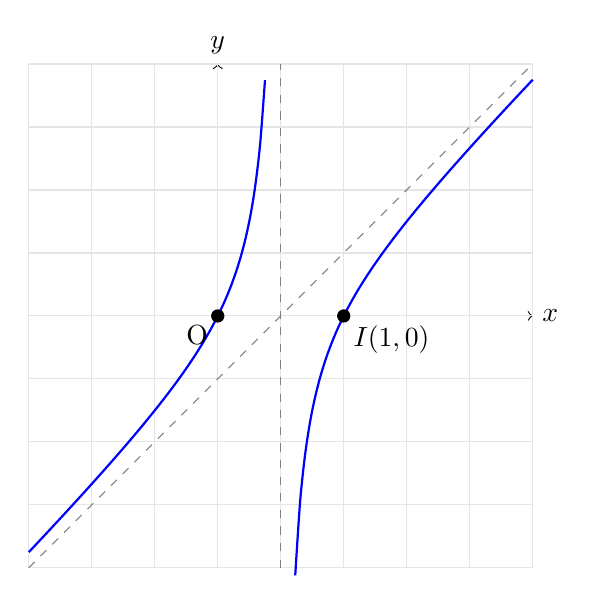
\begin{tikzpicture}[scale=0.8]
    % Hệ trục tọa độ
    \draw[->] (-3,0) -- (5,0) node[right] {$x$};
    \draw[->] (0,-4) -- (0,4) node[above] {$y$};
    % Lưới tọa độ (mờ)
    \draw[gray!20] (-3,-4) grid (5,4);
    % Tiệm cận đứng
    \draw[dashed, gray] (1,-4) -- (1,4);
    % Tiệm cận xiên
    \draw[dashed, gray] plot[domain=-3:5] (\x, {\x-1});
    % Đồ thị hàm số (hai nhánh)
    \draw[blue, thick, smooth, domain=-3:0.75, samples=50] plot (\x, {(\x*\x-2*\x)/(\x-1)});
    \draw[blue, thick, smooth, domain=1.23:5, samples=50] plot (\x, {(\x*\x-2*\x)/(\x-1)});
    % Đánh dấu các điểm đặc biệt
    \fill (0,0) circle (3pt) node[below left] {O};
    \fill (2,0) circle (3pt);
    \node at (2,0) [below right] {$I(1,0)$};
\end{tikzpicture}
\end{document}